\documentclass[12pt]{article}
\usepackage{graphicx, amsmath}
\graphicspath{ {./} }
\setlength{\oddsidemargin}{0.25 in}
\setlength{\evensidemargin}{-0.25 in}
\setlength{\topmargin}{-0.6 in}
\setlength{\textwidth}{6.5 in}
\setlength{\textheight}{8.5 in}
\setlength{\headsep}{0.75 in}
\setlength{\parindent}{0 in}
\setlength{\parskip}{0.1 in}

\begin{document}
\thispagestyle{plain}
   \newpage
   \setcounter{page}{1}
   \noindent
   \begin{center}
   \framebox{
      \vbox{\vspace{2mm}
    \hbox to 6.28in { {\bf BioE 131: Intro to Computational Biology}
                        \hfill Fall 2020 }
       \vspace{4mm}
       \hbox to 6.28in { {\bf \Large \hfill Pairwise Alignment  \hfill} }
       \vspace{2mm}
       \hbox to 6.28in { {\it Professor: Ian Holmes \hfill} }
      \vspace{2mm}}
   }
   \end{center}
   {Notes written by Vikram Shivakumar}
   \vspace*{4mm}


\section{Introduction}
\textbf{Pairwise alignment} involves aligning two sequences (DNA, RNA, or proteins) and is an integral part of computational biology. Many features of nucleic acids and polypeptides derive directly from the sequence, so the ability to compare sequences allows us to better understand problems from protein structure and gene function prediction, to molecular evolution and sequence conversation. In this note, we will explore the uses of sequence alignment in bionformatics, and some algorithms and techniques used to compute alignments.

\section{Why align sequences?}
Sequence alignment is used in various problems across biology, in particular proteomics, genomics, and molecular evolution. To understand the importance of alignment, we'll take a look at a few motivating examples across computational biology.

\subsection{Function Prediction}
The assumption in \textbf{function prediction} is that similar sequences (whether nucleic acid or peptide sequences) tend to have similar function. Though this is not always the case, we can use the function of similar sequences to make a first-order approximation of the function of a gene of interest. We can also align two similar genes with \textit{different} functions to understand how variation in sequence may affect gene function.\\[10pt]
However, there are some complications in using sequence homology alone to assign infer function. For example in a gene duplication, different copies of the same sequence can take on different functions, in which case inferring gene function from sequence similarity would not be possible. Another complication is the presence of \textbf{low-complexity regions}, sequences with simple repeats and low variability in composition (e.g. microsatellites, amino acid repeats). These regions can be similar to other sequences by coincidence, rather than due to homology. These regions can be detected with \textbf{sliding-window entropy filters}, where the entropy along the sequence is calculated, and areas of low entropy (like repeats) can be identified and masked out (i.e ignored) during the alignment.
\begin{figure}[h]
    \centering
    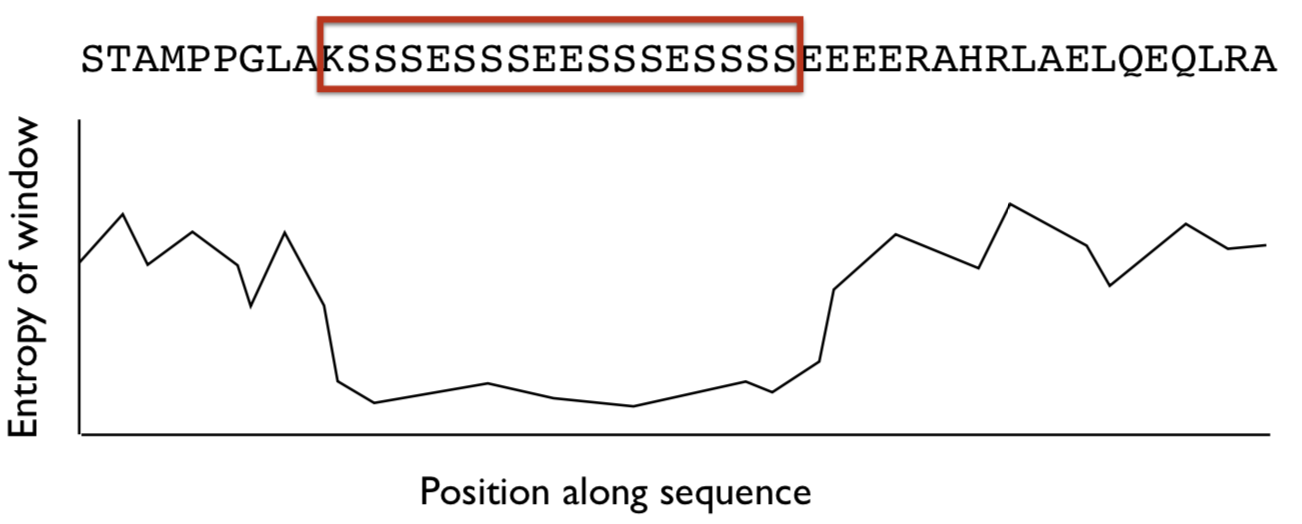
\includegraphics[width=.8\linewidth]{entropy_filter.png}
    \caption{Entropy along an amino acid sequence}
    \label{fig:entropy}
\end{figure}

\subsection{Structure Prediction}
As we saw in the RNA folding module, RNA structure prediction can be done \textit{ab initio}, without aligning RNA sequences. But for proteins, \textit{ab initio} folding (randomly sampling from the protein conformational space) is computationally infeasible! \textbf{Levinthal's paradox} describes this problem, claiming that even sampling a new protein structure every \textit{picosecond} would be too slow to cover the astronomical number of conformations for a single amino acid sequence. For example, for an $N$ length sequence, there are $(2N-2)$ $\Phi$ and $\Psi$ bond angles, each of which could be in $X$ conformations, leading to $X^{2N-2}$ possible structures!\\[10pt]
Thus for proteins, we can use homology to determine structures, taking advantage of the idea that structure is conserved evolutionarily longer than peptide sequence. Although multiple other factors contribute to protein structure (like pH, ions and cofactors, and chaperone proteins), some of the structure can be determined from sequence-dependent factors like polar and nonpolar interactions, disulfide bridges, etc. The \textbf{CASP competition} is a biennial experiment which involves predicting structures of soon to be characterized proteins, to assess the current state of protein structure prediction.

\subsection{Molecular evolution}
Sequence alignment can also be used to identify conserved regions across many sequences within a protein family or within a phylogenetic clade. These conserved elements can be used to identify protein domains or important gene features like exons/introns. For example in genes, introns tend to be more variable than exons, since mutations in exons could disrupt the protein sequence and function. Thus introns and exons can be identified by conserved regions in alignments.\\[10pt]
Sequence evolution and phylogenies can also be reconstructed from aligning multiple sequences and grouping those that are more similar. Alignments can also reveal relationships between genes in a family, as well as the rate of mutations among the sequences.

\section{Algorithms for sequence alignment}
Now let's look at a few methods for aligning sequences. The main algorithms for aligning two sequences involve \textbf{Dynamic Programming (DP)}, similar to  the Nussinov and McCaskill algorithms. We can also visualize alignments using \textbf{dotplots}, similar to the McCaskill plots for RNA structure. We can also adjust how we score an alignment, penalizing certain mismatches or small length gaps more to make the alignment more biologically accurate.

\subsection{Alignment Definitions}
The columns in a \textbf{collinear alignment} represent the alignment of single bases (or amino acids) across the sequences. These columns can fall under two main categories: \textbf{substitutions} and \textbf{indels}. Substitutions can be either matches or mismatches (e.g. mutations), while indels are represented with gap characters (usually "-" or "."). The gaps in an indel can be in either sequence in an pairwise alignment, since an insertion in one sequence could be a deletion in another (often we don't know which sequence is \textit{ancestral}, so the choice is arbitrary).\\[10pt]
We can visualize a collinear alignment with an \textbf{alignment path graph}. The sequences to be aligned are on each axis of the graph, and the path along the graph constitutes the alignment, with diagonals representing substitutions and edges representing gaps.
\begin{figure}[h]
    \centering
    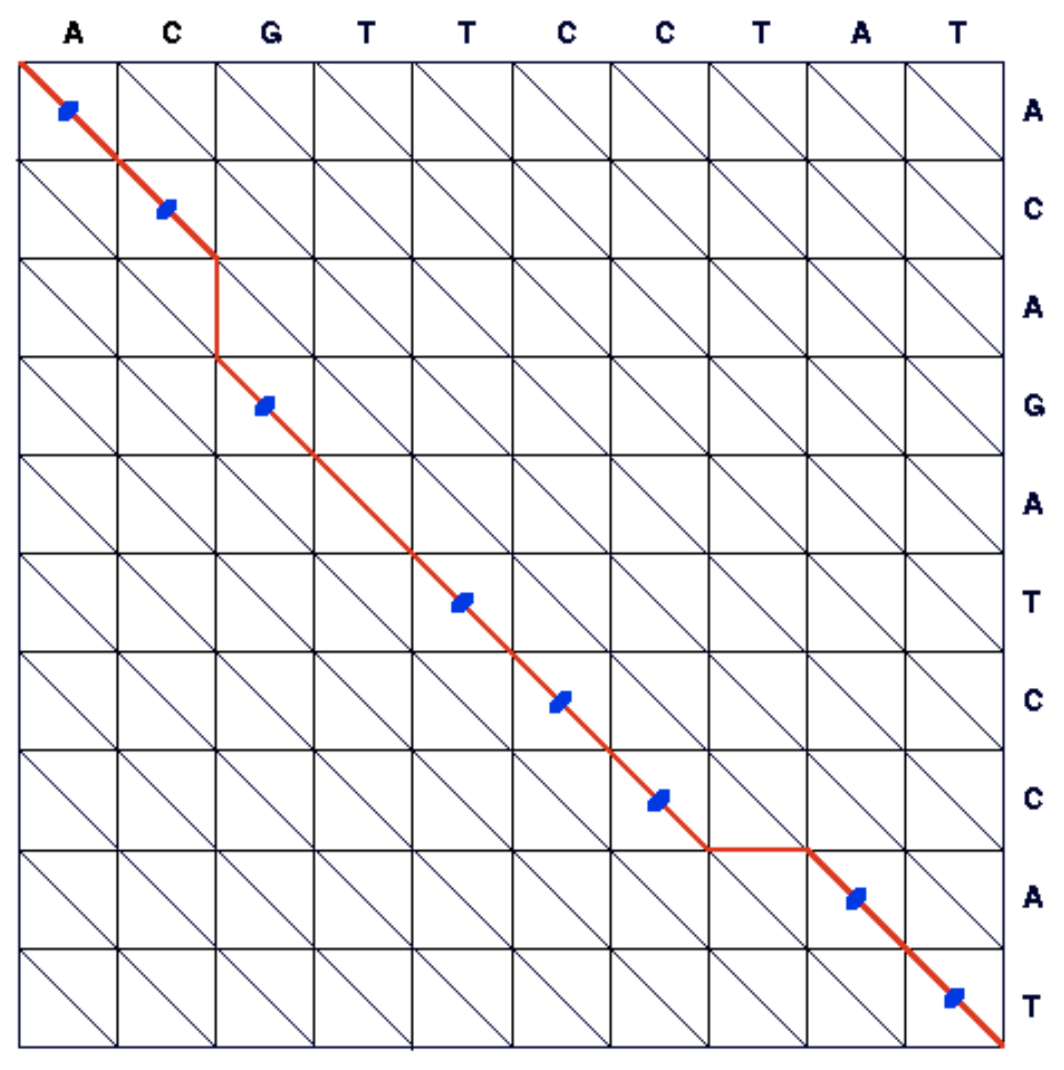
\includegraphics[width=.2\linewidth]{alignment_graph.png}
    \caption{Example of an alignment path graph}
    \label{fig:align_graph}
\end{figure}

Alignments fall into two main types: \textbf{global} and \textbf{local}. Global alignments involve the entirety of both sequences (e.g. aligning two homologous proteins). Local alignments finds the best match between subsequences (e.g. aligning similar domains within two different proteins). A \textbf{semi-local} alignment is global with respect to one sequence (the \textit{query}), and local with respect to the other (the \textit{target}) (e.g. aligning a sequencing read to a reference genome). Each of these scenarios can be represented by a type of alignment graph: 
\begin{figure}[h]
    \centering
    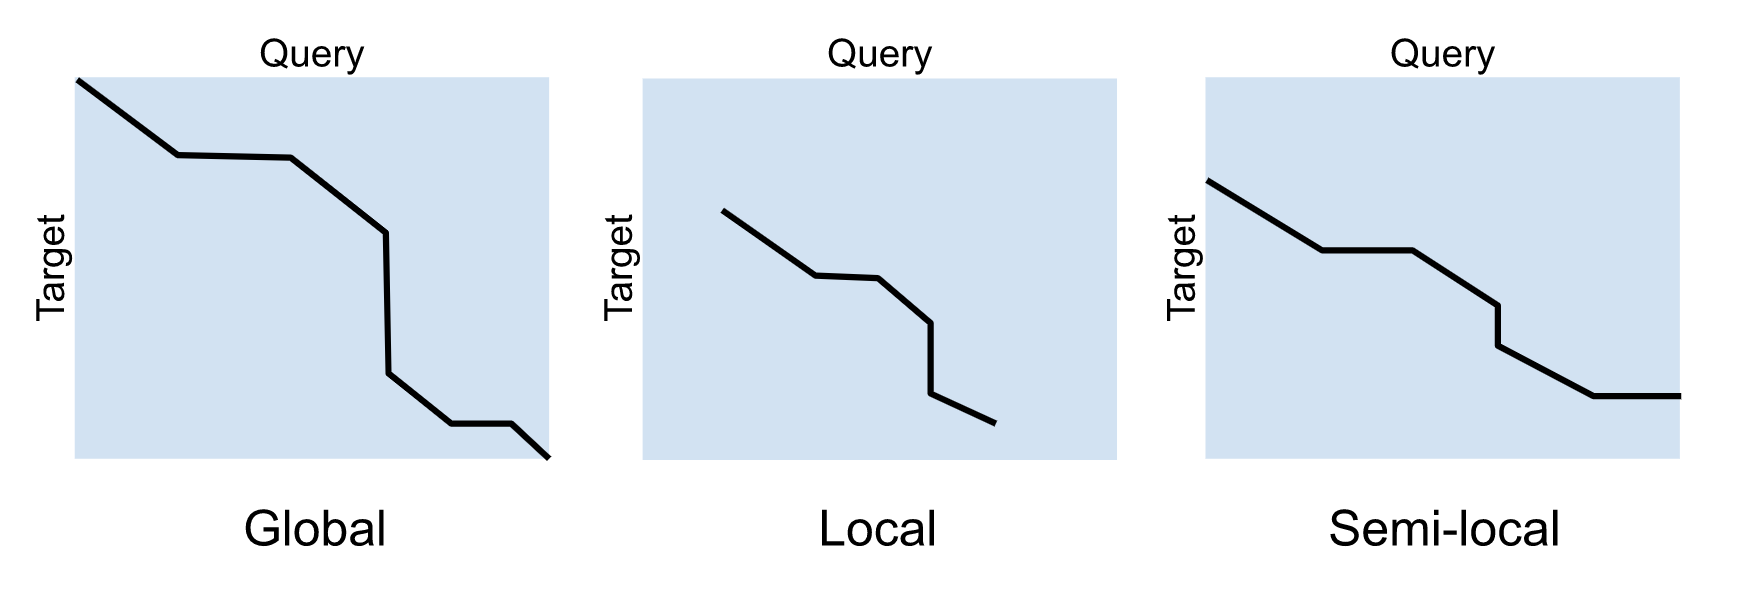
\includegraphics[width=.8\linewidth]{Pairwise-Alignment/global_local.png}
    \caption{Alignment path graphs for global, local, and semi-local alignments}
    \label{fig:global}
\end{figure}

\subsection{Dotplots}
Dotplots can be used to visualize an alignment of two sequences. The sequence is represented along an axis, and a dot at coordinate $(i,j)$ represents an alignment between the $i$th character in sequence $X$ and $j$th character in sequence $Y$.\\[10pt]
Dotplots can also be used to identify specific regions of an alignment like perfect matches, palindromes, and indels (see Figure \ref{fig:dot}). 
\begin{figure}[h]
    \centering
    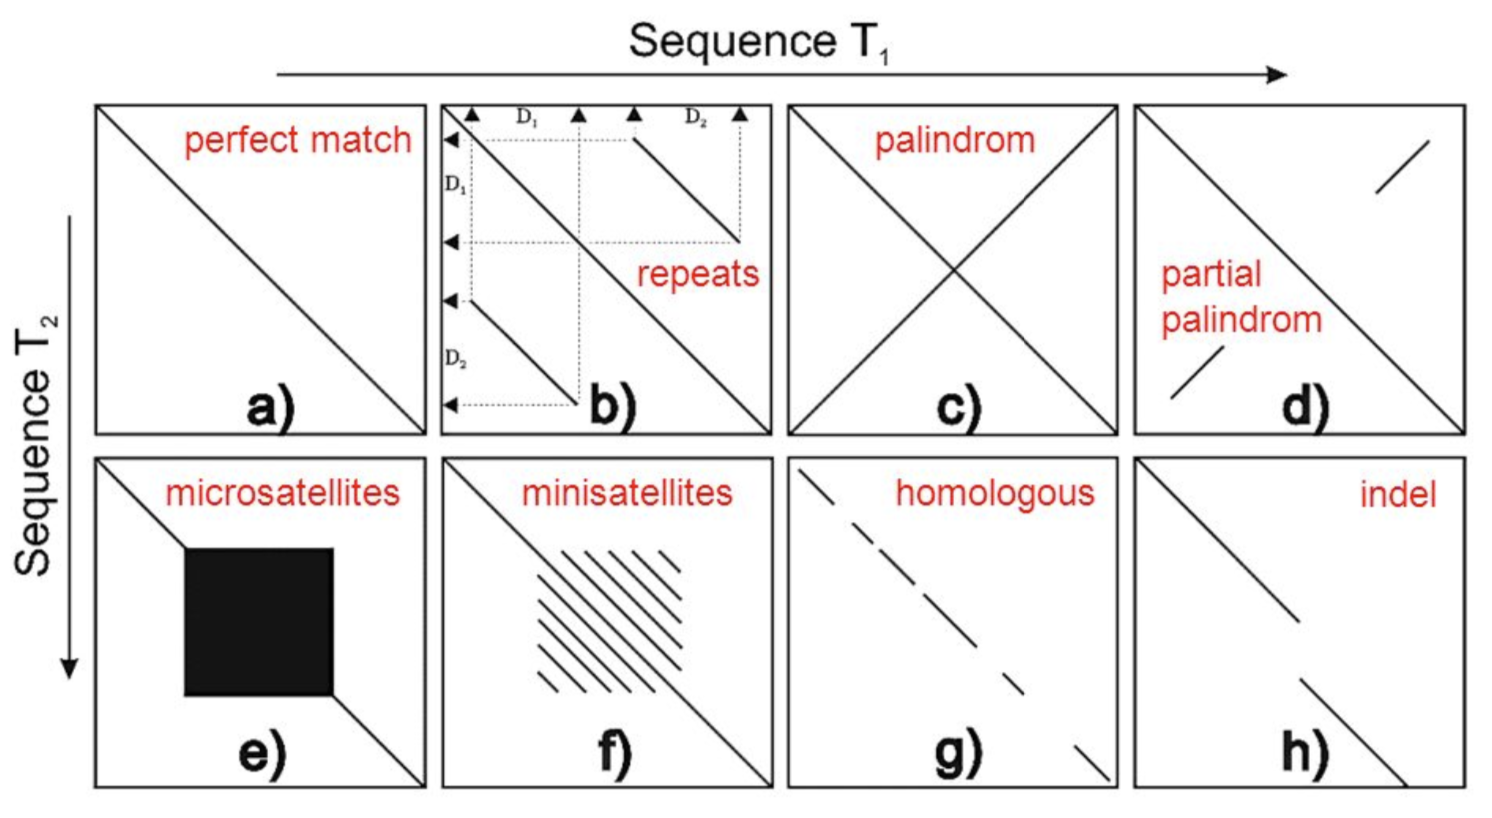
\includegraphics[width=.8\linewidth]{seq_dot.png}
    \caption{Types of alignment regions in dotplots}
    \label{fig:dot}
\end{figure}
We can also construct a dotplot of a sequence to itself (similar to a McCaskill plot), where stretches of dots would represent repeatetive sequences.

\subsection{Scoring Schemes}
\subsubsection{Edit Distance}
To build algorithms for constructing alignments, we need a way to score an alignment (which we can then optimize to find the best alignment). The most basic way of scoring a collinear alignment is \textbf{edit distance}, a concept from computer science. One type of edit distance, \textbf{Hamming distance}, penalizes each mismatch with a point. The \textbf{Levenshtein distance} is similar to Hamming distance, but also includes single point penalties for gaps. Thus to find the best alignment, we would need to minimize the edit distance.\\[10pt]
However not all substitutions are equally likely, so we should not uniformly penalize them. For example, a transversion (purine to pyrimidine and vice-versa) should be penalized \textit{more} than a \textbf{transition} (purine to purine or pyrimidine to pyrimidine), as transitions are more likely. To store the penalties for each substitution, we can create a \textbf{substitution matrix}, which contains the scores for all combinations of substitutions (the score for a match could be 0 or even negative). One example is the \textbf{BLOSUM62 matrix}, which defines scores for each amino acid substitution based on frequencies derived from observed alignments
\subsubsection{Log Odds Ratio}
The scores in the BLOSUM62 matrix are \textbf{log odds ratio} scores, which we can define as $Q(X_i,Y_i)$:
$$\sum_{i=1}^LQ(X_i,Y_i) = \sum_{i=1}^L\log \frac{P\left(X_i,Y_i\right)}{P\left(X_i\right)P\left(Y_i\right)} = \log\prod_{i=1}^L\frac{P\left(X_i,Y_i\right)}{P\left(X_i\right)P\left(Y_i\right)} = \log\frac{P\left(X,Y\right)}{P\left(X\right)P\left(Y\right)}$$
The ratio of probabilities is the \textbf{odds ratio}, and by taking the log, we can find the odds ratio of a whole alignment by taking the sum. The odds ratio is the ratio of an alignment column \textit{together}, divided by the individual probabilities of each character. The log odds ratio is related to the concept of mutual information between two sequences.
\subsubsection{Gap Penalties}
Finally, we can modify gap penalties to make alignments more biologically realistic. In the case of edit distances, each gap is penalized equally, however in DNA, RNA, and proteins, gaps tend to be multiple characters long, rather than small interspersed gaps. To model this, we can use an \textbf{affine gap penalty}, as opposed to a \textbf{linear} penalty, where the cost of the first gap is larger than subsequent, consecutive gaps. Thus, gaps will only be introduced into an alignment where longer stretches are required, otherwise substitutions are preferred.

\section{Dynamic Programming Algorithms}
Now let's look at some dynamic programming algorithms that are used 
to create alignments between two sequences. 
\subsection{Needleman-Wunsch algorithm}
The Needleman-Wunsch algorithm is used for global alignments between two sequences and uses a linear gap penalty. Similar to algorithms for RNA folding, we use dynamic programming to iteratively evaluate subproblems towards a final solution. In Needleman-Wunsch, the idea is that there are 3 options for the final column of a collinear alignment between sequences $X$ and $Y$:
\begin{enumerate}
    \item A substitution (match or mismatch)
    \item A gap in sequence $X$ 
    \item A gap in sequence $Y$ 
\end{enumerate}
In case (1) we can then find the best alignment of the remaining sequences $X_{i-1}$ and $Y_{i-1}$, plus the score $Q(X_i,Y_i)$ from a substitution matrix. In case (2) we can find the best alignment between $X_{i}$ and $Y_{i-1}$, and likewise between $X_{i-1}$ and $Y_{i} $for case (3), adding the penalty for a gap, $G$. Formalizing this recursion into an equation, where $S_{i,j}$ is the best alignment between $X_i$ and $Y_j$:
\begin{equation*}
S_{ij} = \max\begin{cases}
S_{i-1, j-1} + Q(X_i,Y_j) &\text{if }i>0, j>0\\
S_{i-1, j} - G &\text{if }i>0\\
S_{i, j-1} - G &\text{if }j>0\\
0 &\text{if }i=j=0\\
\end{cases}
\end{equation*}
To find the best score for the full alignment, we just need to calculate $S_{L,M}$, where sequence $X$ is of length $L$ and sequence $Y$ of length $M$. To do this, we fill in a dynamic programming table, where value $(i,j)$ represents $S_{i,j}$, and is calculated using the values in $(i-1,j-1)$, $(i-1,j)$, and $(i,j-1)$, representing each case. After calculating the value of $S_{i,j}$, we can store a pointer to the case which yielded the max value. Then to retrieve the actual alignment, we can retrace from $S_{L,M}$ through each pointer to $S_{0,0}$.
\begin{figure}[h]
    \centering
    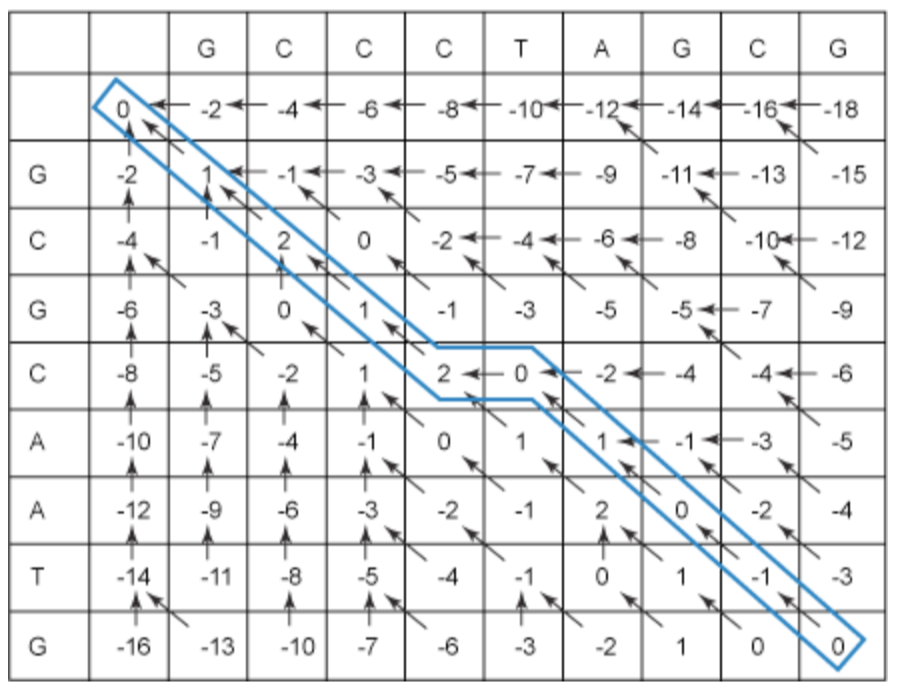
\includegraphics[width=.6\linewidth]{needleman.png}
    \caption{Example of a DP table and traceback for Needleman-Wunsch}
    \label{fig:needle}
\end{figure}
\subsection{Smith-Waterman algorithm}
The Smith-Waterman algorithm is a variation of the Needleman-Wunsch algorithm for local alignments. Using a similar recursion, we can achieve a local alignment by adding a new case: each item $S_{i,j}$ in the DP table can also come directly from the start, with a value of 0:
\begin{equation*}
S_{ij} = \max\begin{cases}
S_{i-1, j-1} + Q(X_i,Y_j) &\text{if }i>0, j>0\\
S_{i-1, j} - G &\text{if }i>0\\
S_{i, j-1} - G &\text{if }j>0\\
0 &\\
\end{cases}
\end{equation*}
In this new algorithm, the final solution is not $S_{L,M}$, but instead the max value of the DP table: $$\max_{0\leq i\leq L, 0\leq j\leq M} S_{i,j}$$
Thus during traceback, we start at the max value in the DP table, and follow the pointers until a value points back to the start (in case (4)).
\subsection{Gotoh algorithm}
The Gotoh algorithm extends Smith-Waterman and Needleman-Wunsch further to include affine gap penalties. It can do both global and local alignments (just need to modify Needleman-Wunsch vs Smith-Waterman), but we will look at the global alignment version for now.\\[10pt]
In cases (2) and (3), we need to modify the current recursion in case we are \textbf{opening} or \textbf{extending} a gap. For this, we can build 2 separate DP tables: $T_{i,j}$ representing the best alignment between $X_i$ and $Y_i$ \textit{ending in an alignment}, and $U_{i,j}$ representing the best alignment between $X_i$ and $Y_i$ \textit{ending in a gap}. Then in table $T$, we can calculate a value $U_{i,j}$ using previous values from both $T$ and $U$ depending on if we are closing a gap or not.\\[10pt]
We can also think of Gotoh as a \textbf{finite state machine}, where we alternate between a $T$ and $U$ state, and we have multiple self loops. Moving from state $T$ to $U$ requires an opening gap penalty $G$, and in reverse an extension penalty $E$.
\begin{figure}[h]
    \centering
    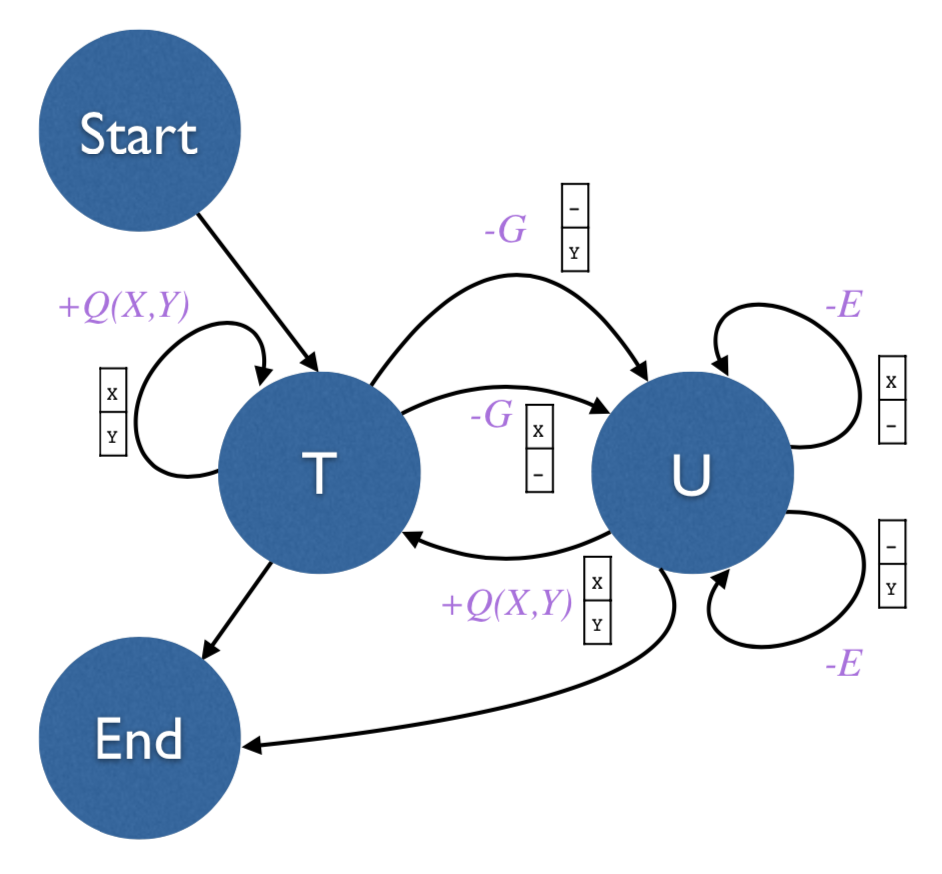
\includegraphics[width=.6\linewidth]{gotoh_state.png}
    \caption{Example of a Gotoh finite state machine}
    \label{fig:gotoh}
\end{figure}

\subsection{Runtime and Space Complexity}
As with any algorithm, let's look at the time and space complexity. For Needleman-Wunsch, we use a 2D DP table, thus the space complexity would be $O(LM)$, where sequences $X$ and $Y$ are length $L$ and $M$ respectively. The runtime complexity would also be $O(LM)$ since we are calculating a value for each entry in the table, and thus iterate through all combinations $(i,j)$. However we can improve the space complexity by observing that we only need values from the current and previous row to calculate any particular value. Thus we can just store 2 lines at a time, or $O(\min (L,M))$. However, this improvement in space complexity comes at a cost, as now we cannot store pointers and run a traceback to get the full alignment (we can only compute the best alignment score). One way to compute the full alignment while improving space complexity is to use a \textbf{divide and conquer approach}, which yields a space complexity of $O(\min(L,M)\log \min(L,M))$. This however increases the time complexity to $O(LM\log \min(L,M))$. These complexities also apply to Smith-Waterman, since the DP recursion is similar. The Gotoh algorithm uses two DP tables, but this only increases the complexities by a constant factor, so the Big-O complexities are the same as well.\\[10pt]
\textit{Note}: Often, the length of both sequences are considered to be comparable, in which case the complexity simplifies a bit. For example, the runtime and memory complexities of Needleman-Wunsch would simplify to $O(L^2)$ in the basic case (and likewise instead of the $min(L,M)$ terms in the other cases, we can simplify to just $L$).

\section{BLAST}
The \textbf{Basic Local Alignment Search Tool}, or \textbf{BLAST}, is a tool used to align a sequence to a large database of sequences. If the database contains many sequences, running a pairwise alignment on the query and every possible database entry is computationally infeasible. BLAST uses a couple of techniques (kmer searches, database indexing, constrained DP) to efficiently find high scoring matches for the query sequence. The BLAST algorithm has a few steps:
\begin{enumerate}
    \item Split the query into a list of kmers, and add similar kmers (incorporating possible substitutions using for example a BLOSUM matrix)
    \item Find matches of kmers in a sequence index
    \item Extend matches by connecting nearby kmer matches into \textbf{high scoring segment pairs (HSP)}
    \item Evaluate the significance of the HSPs (using an extreme value distribution)
    \item Connect HSPs to form the full alignment using constrained DP
\end{enumerate}
Allowing substitutions in the kmer list lets the algorithm find non-exact matches to the query. These kmers are then searched in an \textbf{sequence index}. An example of an index is a \textbf{suffix tree}, which encodes all the possible suffixes (or subsequences) of a sequence in a tree format, allowing for efficient querying of a suffix. Another example \textbf{FM index}, which uses the Burrows-Wheeler transform to compress sequences. Lastly some hash schemes can be used to efficiently query an index for a query kmer.\\[10pt]
Once the kmers are searched across the index, matches that are close are connected into HSPs. These HSPs can then be evaluated using an EVD (see the note on probability distributions), and significant HSPs can be connected into a final alignment. This is done using \textbf{constrained DP}, where dynamic programming is used on the query and target sequence, with the constraint that the path through the DP matrix must go through the areas containing these HSPs (which is more efficient that a full DP).
\section{Summary}
Sequence alignment is used across computational biology to solves problems, and various algorithms exist to efficiently compute alignments. Some algorithms like Needleman-Wunsch, give exact solutions, but can be computationally expensive in some cases. Others, like BLAST, provide alignment results more efficiently using techniques to avoid computing a full alignment. These algorithms are essential to understanding problems of sequence homology, molecular evolution, and protein structure, as well as non-biological problems in linguistics and computer science.
\end{document}


%topics not covered:
%examples of various insights revealed by alignment
%bayesian inference with log odds
%include recursion equation for GOtoh?
%BLAST, not yet
